\chapter{Research Methodology}
\label{chap:method}
This chapter presents the research method used in this thesis. Firstly, the research motivation is presented, followed by the research questions defined for this thesis. The research method and design are explained in the third section. The fourth section presents an overview of the research implementation. Finally, the fifth section presents the various tools and libraries used for this thesis.

\section{Research Motivation}
Writing Smart Contracts are hard. Writing secure Smart Contracts is even harder. Automatic code generation is by many considered the ”holy grail” in the field of computer science \cite{PGL-010}. Recent works have applied transformers for code generation and program synthesis, achieving state-of-the-art results. For example, Codex by \cite{chen2021codex} fine-tunes GPT-3 \cite{brown2020language} on code data from GitHub. The results are impressive. However, these systems still face many problems, especially in regards to different biases, for example, gender and security biases. Because the model is trained on open-source code \cite{chen2021codex}, including "Public code may contain insecure coding patterns, bugs, or references to outdated APIs or idioms.", the model might "synthesize code that contains these undesirable patterns introduce vulnerabilities" \cite{copilot}. An empirical study by \textcite{pearce2021asleep} found that almost approximately 40\% of the generated code by GitHub Copilot is vulnerable. Security flaws in software results yearly in loss of tens of thousands of million dollars\todo{find real number here .}. Due to the monetary nature of blockchain, security flaws are even more severe, as exploits of vulnerabilities often directly result in the loss of funds. Further, the immutable nature prevents the possibility of correcting vulnerable code after being deployed. Therefore, the research objective is to develop a system that can generate secure smart contract code automatically, without the need for human intervention. \todo{Rewrite}. This thesis tries to address the above problems by answering the research questions defined in \cref{sec:research-questions}. this includes both investigating how 


\section{Research Questions}
\label{sec:research-questions}
The research questions addressed in this thesis are:

    

\begin{enumerate}[label=\textbf{RQ\arabic*.}, leftmargin=1.5cm]
    \item How to automatically generate smart contract code with transformer-based language models?
    \begin{enumerate}[label*=\textbf{\arabic*.}]
        \item How well do pre-trained transformer-based language models work for smart contract synthesis? \todo{compare to literature review in chapter: related-works}
        \item What impact does fine-tuning a transformer model on smart contract code have on its code generation ability?
    \end{enumerate}
    \item How to generate secure code with transformer-based language models?
    %\item How to reduce the vulnerability bias in the transformer model.
    \item How to best construct inputs for automatic code generation?
\end{enumerate}

\section{Research Method and Design}
\label{sec:research-method-and-design}

The underlying foundation for how research is conducted is rooted in the research philosophy used. For this research, a positivistic research philosophy was used. A positivistic philosophy assumes that the world is not random, that it is ordered and regular, and that one can investigate it objectively. \todo{Cite - B. J. Oates, Researching information systems and computing, Sage, 2006.} A deductive research approach was used. To best facilitate the answering of the research questions defined in \cref{sec:research-questions}, experiments were selected as the research strategy. These experiments included fine-tuning pre-trained language models, as well as testing these on real data and man-made data. The results from the evaluation of the fine-tuned models are recorded as observations and quantitatively evaluated.




%The research is conducted objectively. It is based on facts that are repeatable and quantitatively evaluated. 


%Research Philosophy - positivism
%Research Type - inductive (exploratory) + Quantitative
%Research Strategy - experiments (train and test)
%Time Horizon- one-time data set construction (1st of april)
%Sampling Strategy  - probability sampling (random)
%Data Collection Method - Observation? Evaluate performance
%Data Analysis Methods - Employ primarily a quantitative analysis, as well as some qualitative analysis. (mixed methods?)


\section{Research Implementation}
\label{sec:research-implementation}

For the implementation of the research, first, the datasets needed for the experiments were constructed. The datasets creation phase is divided into the following steps:
\begin{enumerate}
    \item Create verified smart contract source code dataset.
    \begin{enumerate}
        \item Scrape verified smart contracts from the Ethereum blockchain.
        \item Filter scraped verified smart contracts for uniqueness.
    \end{enumerate}
    \item Create an audited version of the smart contract dataset
    \begin{enumerate}
        \item Label the smart contracts with a vulnerability detection tool.
    \end{enumerate}
    \item Create a parsed dataset containing "comment, function" pairs. This will facilitate testing, as well as research question 3.
    \begin{enumerate}
        \item Create a parser that can parse all contract versions.
        \item Parsing the verified smart contracts with a parser.
    \end{enumerate}
\end{enumerate}
A comprehensive description of the creation of the datasets used in this project is given in \cref{chap:datasets}.
\newline
\newline
Secondly, the language modeling process is divided into 2 phases:
\begin{enumerate}
    \item Fine-tune a transformer model on the verified smart contracts dataset.
    \item Fine-tune a transformer model on the audited verified smart contract dataset, employing security conditioning.
\end{enumerate}
A comprehensive description of the implementation of the language models is given in \cref{chap:language-modeling}.

\section{Plan of the Experiments}
This section presents the plan for how the experiments in \cref{chap:experiments-and-results} are executed. This includes an overview of the different technologies applied, both software and hardware, as well as the different phases of the experiments.

\subsection{Technology}
\label{sec:technology}

\subsection{Software}
\label{sec:software}
During the selection of the language modeling library for use in this project, several considerations were made. Firstly, due to the huge size of the model, the library needed to support distributed GPU training. It had to be flexible and scalable, without sacrificing too much on speed. The transformers \cite{transformers} library by Hugging Face \cite{hugging-face} fulfilled these conditions. The library provides flexible and easy-to-use solutions. It also supports integration with DeepSpeed \cite{deepspeed}, a deep learning optimization library by Microsoft \cite{microsoft} that makes distributed training and inference easy, efficient, and effective. The Hugging Face ecosystem also provides the Datasets and Tokenizers libraries, streamlining and significantly simplifying the use of large datasets.

\subsection{Hardware resources}
\label{sec:hardware-resources}

IDUN High Performance Computing Platform

\begin{figure}[htp]
    \centering
    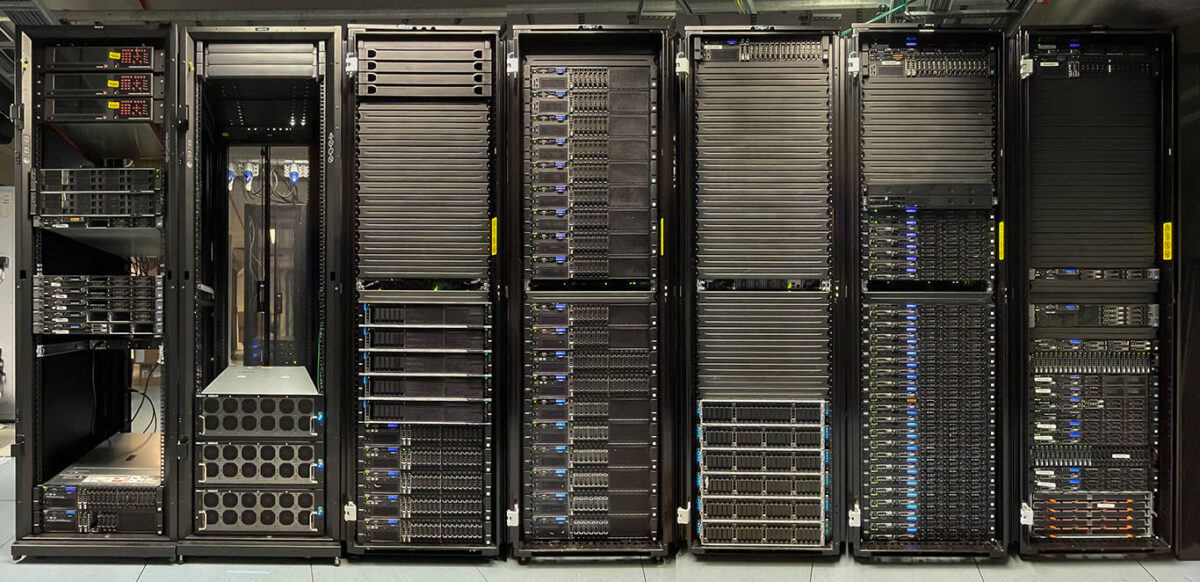
\includegraphics[width=\textwidth]{figures/idun.jpeg}
    \caption{Image of IDUN todo: add ref \url{https://www.hpc.ntnu.no/idun/}}
    \label{fig:flowchart}
\end{figure}

\subsection{Experimental process}
\label{sec:experimental-process}
This project employs an experimental and analytical research method, as described in \cref{sec:research-method-and-design}. The standard scientific method was used for all the experiments. This included stating a hypothesis, implementing the required systems, executing the experiments, and evaluating the results. Several metrics were used to evaluate the results. For evaluating the performance of the smart contract generation, accuracy, BLEU score and Perplexity were used. 

in addition to the standard deviation when conducting statistical hypothesis tests.

These experiments included fine-tuning pre-trained language models, as well as testing these on real data and man-made data

\subsection{Project scope}
\label{sec:project-scope}

The project scope in this thesis is limited to the generation of smart contracts for the Ethereum blockchain. Further, only one language model architecture is used. Specifically, the state-of-the-art open-sourced pre-trained transformer model GPT-J-6B by ElutherAI is selected. For research questions 1 and 2, two versions of the model were created by fine-tuning it on two smart contract datasets created for this project. Due to the share size of this model (see \cref{sec:requirements}), no hyper-parameter optimization was performed. The hyper-parameters were left to defaults used during pre-training. Hence, everything but the training data is keept constant throughout the experiments. For research question 3, the primary scope is to assess variations in the actual input to the model. Thus, differences in performance due to variations of the models' inference configuration are not thoroughly explored.
